\documentclass{article}

\usepackage{epsfig}
\usepackage[mathscr]{eucal}
\usepackage{amsfonts}
\usepackage{amscd}
\usepackage{amsmath}
\usepackage{array}
\usepackage{amssymb}
%\usepackage[backend=bibtex8, sorting=none]{biblatex}
\usepackage{colordvi}
\usepackage{enumerate}
\usepackage{graphicx}
\usepackage{booktabs}
\usepackage[footnotesize]{caption}
\usepackage{fancyhdr}
\usepackage{pdfpages}
\usepackage{slashed}
\usepackage{tabularx}
\usepackage{longtable}
\usepackage{array}
\usepackage{caption}
\usepackage{subcaption}

%\usepackage{relsize}
\usepackage{color}
\usepackage{rotating}

\usepackage{slashed}

\usepackage{epsfig,amsmath,graphicx,amssymb,listings,slashed}
\usepackage[colorlinks,citecolor=blue,urlcolor=blue,linkcolor=blue]{hyperref}
\usepackage[outercaption]{sidecap}

\usepackage{booktabs}

%\smartqed
%\usepackage[T1]{fontenc}
\usepackage[utf8]{inputenc}

\usepackage{epsfig,amsmath,graphicx,amssymb,listings,slashed}
\usepackage[colorlinks,citecolor=blue,urlcolor=blue,linkcolor=blue]{hyperref}

\setlength{\evensidemargin}{0cm}
\setlength{\oddsidemargin}{0cm}
\setlength{\topmargin}{0.00cm}
\setlength{\textwidth}{16.0cm}
\setlength{\textheight}{24.00cm}
\setlength{\headheight}{0cm}
\setlength{\headsep}{0cm}
\setlength{\voffset}{0cm}
\setlength{\paperheight}{29cm}

\definecolor{ourbrown}{RGB}{155,100,15}
\definecolor{ourcyan}{RGB}{20,165,165}
\definecolor{ourpurple}{RGB}{145,0,140}
\definecolor{darkorange}{RGB}{225,100,0}
\definecolor{darkgreen}{RGB}{0,170,0}
\definecolor{darkgray}{RGB}{80,80,80}

\setlength{\marginparwidth}{20mm}







\begin{document}

\title{ Machine Learning - SS 2021 \\ Exercise 1: Classification }


	\author{Federico Ambrogi, \textcolor{blue} {e1449911@student.tuwien.ac.at } \\
	Adam Höfler, \textcolor{blue} {e11847620@student.tuwien.ac.at } \\
	Matteo Panzeri \textcolor{blue}{12039996@student.tuwien.ac.at } \\
    TU Wien }


%\ead{federico.ambrogi@univie.ac.at}




\maketitle
\setcounter{tocdepth}{2}
\tableofcontents

\section*{Introduction}
In this document we describe the results of the implementation of three algorithms to solve classification problems on four different dataset. 



\section{Data Sets Description}
Here we briefly introduce our four datasets.
\paragraph{Drug consumption data set} This is the data set taken from exercise 0, so here we only provide basic details. The primary task of our implementation is to classify the likeliness of the frequency of usage of a certain type of drug (from never used to current usage), given personal aspects such as gender, ethnicity, education background etc. and psychological traits.  

\paragraph{Asteroids data set} 
The asteroids data set is designed to perform a binary classification task. It consists of a total of {\color{red} XXX } features, mostly astrophysical parameters of asteroids such as the distance from the Earth, the size of the major axis of the orbits, their mass etc. as well metadata regarding their name. The target feature for classification is a string variable that maps to boolean values "True" in the case the asteroid represents a concrete hazard for the Earth i.e. with high risk of impact, and "False" otherwise.



\paragraph{} 
Blah
\paragraph{} 
Blah

\section{Data Exploration and Pre-processing}
In this section we describe the necessary preliminary steps to import and prepare the data to make them suitable for the learning algorithms.
The steps are handled by the script \textit{data\_preparation.py} which includes dedicated function to pre-process each data set.

\subsection{Asteroids Data Set}
The original data set contained 40 columns of different variable types (numeric and categorical). However, some columns were unnecessary, not usable or redundant for classification purposes, or contained constant values. 



\section{Holdout and Cross Validation}
Here we describe briefly the techniques of "holdout" and "cross validation" that are used to evaluate a model. The \textbf{holdout} method is essentially based on the splitting on the input data set into two subset, one used for training the model, and one used for testing the model, for example in $80\%-20\%$ proportion, although there is not fix recipe for this split. Once the model is trained, the evaluation can be performed on the test data set, and this is therefore possible to check if the prediction of the model match the data. One big issue of this model is that the training strongly depend on the splitting of the initial data set, for example if the characteristic of the training data set are not representative of the whole data set. 

A more powerful method is the \textbf{cross-validation} or "k-fold cross validation". Form the full dataset, a test is held out for final evaluation, but the validation set is no longer needed. For this, the training set is split into $k$ sets, so that the model is trained using $k-1$ folds as training data, and the remaining one is used for the validation as a test set (to compute the interesting metric of the model).
Once we obtain such $k$ number of metrics, the final result is the average of these parameters, obtained for each iteration of the cross-validation on each distinct fold. 








\section{Performance Tests}

\paragraph{Confusion Matrix}
For each classifier, we produce a confusion matrix where each entry $i,j$ corresponds to the number of observations in group $i$, but predicted to be in group $j$. We chose to normalize the entries according to the sum of each row.  
In case of binary classification, the matrix reduces to the number of true negatives ($TN$), false positives ($FP$), false negatives ($FN$) and true positives ($TP$). 

Examples can be see in Fig. \ref{confusion_matrices}.

We remind here the definition of the metric parameters we will used to quantify the performance of our classifiers i.e. precision ($P$), recall ($R$) , accuracy ($A$) and specificity $S$:

\begin{equation}
P = \frac{TP}{TP + FP} \ \ \ \ \ \ \ \  R = \frac{TP}{TP + FN} \ \ \ \ \ \ \ \  A = \frac{TP + TN}{#all} 
\ \ \ \ \ \ \ \  S = \frac{TN}{TN + FP}
\end{equation}

It is straightforward to calculate these parameters for binary classification tasks out of the confusion matrix. In case of multiple labels, we need to calculate these parameter for each class, given that:
\begin{enumerate}
	\item  $TPs$ are the values in the diagonal; \
	\item  $FNs$ for a certain class are the sum of values in the corresponding row excluding the $TP$; \
	\item  $FPs$ for a certain class are the sum of values in the corresponding column excluding the $TP$; \
	\item  $TNs$ for a certain class are the sum of all rows and columns, excluding the class's column and row. \	
\end{enumerate}


Another convenient metric, particularly because it is calculated directly from the proper \textit{scikit-learn} function, is called $f1-score$, which is defined as the harmonic mean of the precision and recall:
\begin{equation}
f1-score = 2 \times \frac{P \dot R }{P + R } 
\end{equation}



\begin{figure}[h!]
	\centering
	\begin{minipage}[b]{0.49\textwidth}
		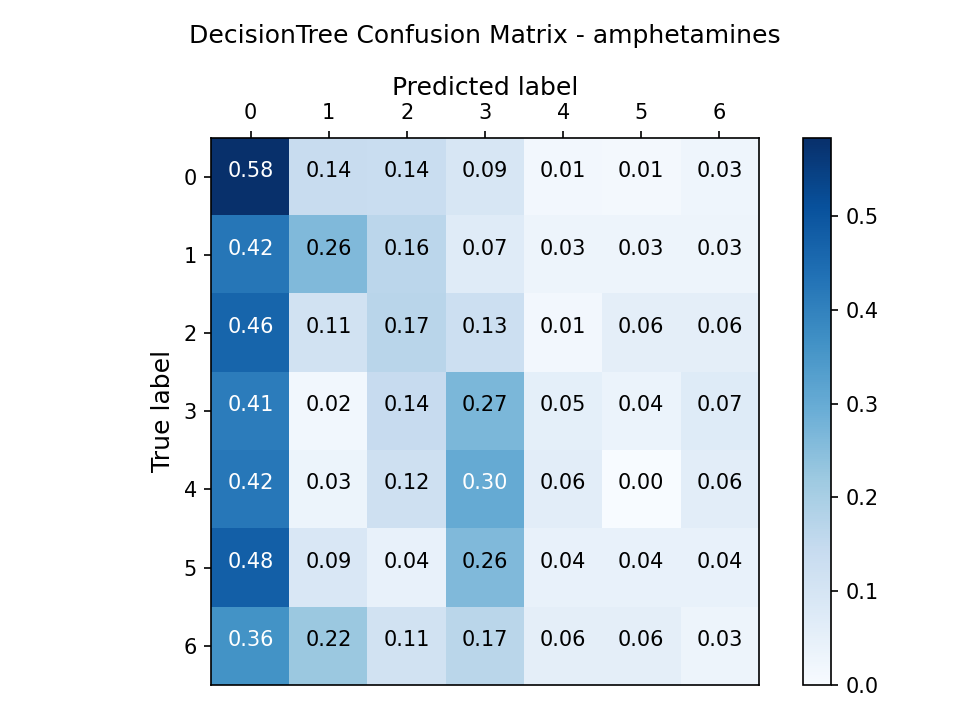
\includegraphics[width=\textwidth]{plots/m2.png}

	\end{minipage}
	\begin{minipage}[b]{0.49\textwidth}
		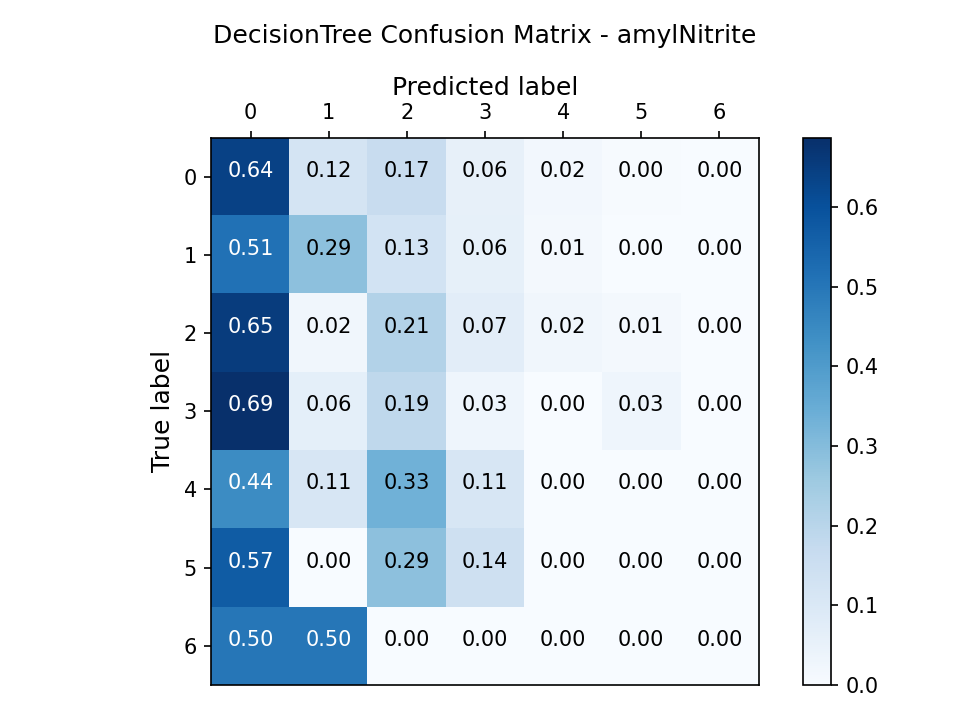
\includegraphics[width=\textwidth]{plots/m1.png}

	\end{minipage}

	\caption{Example confusion matrices for {\color{red} XXX }  }
	\label{confusion_matrices}
\end{figure}


{\color{red} Describe micro averaging and macro averaging, will we report both ? }


\clearpage
\bibliography{literature.bib}{}
\bibliographystyle{unsrt}

\end{document}
